% The entire content of this work (including the source code
% for TeX files and the generated PDF documents) by 
% Hongxiang Chen (nicknamed we.taper, or just Taper) is
% licensed under a 
% Creative Commons Attribution-NonCommercial-ShareAlike 4.0 
% International License (Link to the complete license text:
% http://creativecommons.org/licenses/by-nc-sa/4.0/).
\documentclass{article}

% My own physics package
% The following line load the package xparse with additional option to
% prevent the annoying warnings, which are caused by the package
% "physics" loaded in package "physicist-taper".
\usepackage[log-declarations=false]{xparse}
\usepackage{physicist-taper}

\title{Solution for HW9}
\date{\today}
\author{Taper}

\begin{document}
\maketitle
\abstract{
\begin{CJK}{UTF8}{gbsn}陈鸿翔(11310075)\end{CJK}
}
%\tableofcontents
\section*{Problem 1}
For any smooth function $f$ of $\vec{x}$, we have
$$\bra{\vec{x}}f(\hat{\vec{x}})\ket{\vec{x'}}
= \bra{\vec{x}} \sum_{n=0}^\infty c_n \hat{\vec{x}}^n \ket{\vec{x'}}
= \sum_{n=0}^\infty c_n \vec{x}^n \delta(x-x')
= f(\vec{x})\delta(\vec{x}-\vec{x}')$$

Also use the equation (190) in the lecture notes:
\begin{equation}
    \bra{\vec{x}}\frac{P^2}{2m}\ket{\psi}
    =-\frac{\hbar^2}{2m} \laplacian \braket{\vec{x}|\psi}
\end{equation}
The Schr\"odinger's equation gives

\begin{align*}
    i\hbar\frac{\partial }{\partial t}\braket{\vec{x}|\psi}
    &= \braket{\vec{x}|H|\psi} \\
    &= \bra{\vec{x}} \frac{P^2}{2m}+V(\vec{x}) \ket{\psi} \\
    &= -\frac{\hbar^2}{2m} \laplacian \braket{\vec{x}|\psi} +
    \int\dd{\vec{x}'}\bra{\vec{x}}V(\vec{x})\ket{\vec{x}'}
        \braket{\vec{x}'|\psi} \\
    &= -\frac{\hbar^2}{2m} \laplacian \braket{\vec{x}|\psi} +
        \int\dd{\vec{x}'}V(\vec{x})\delta(\vec{x}-\vec{x}')
        \braket{\vec{x}'|\psi} \\
    &= -\frac{\hbar^2}{2m} \laplacian \braket{\vec{x}|\psi} +
        V(\vec{x}) \braket{\vec{x}|\psi}
\end{align*}

Identifying $\psi(\vec{x},t)$ and $\ket{\vec{x}|\psi}$, then the above
equation is just the normal wave equation (263).

\section*{Problem 2}
For simplicity, take $H_{11}=H_{22}=0$. Then
\begin{equation}
    H= \begin{pmatrix}
        0 & H_{12} \\ 0 & 0
    \end{pmatrix}
\end{equation}
This matrix has rank $1$, so it does not have a full
eigenvector-spectrum.
In addition, its eigenvalues are find by solving characteristic
equation to be $0$, which are not valid eigenvalues. So it does not
have energy eigenstates. This means that the Hamiltonian is not
likely to be physical.

For example, let's solve the Schr\"odinger's equation:
\begin{align*}
    i\hbar\frac{\partial }{\partial t}
    \begin{pmatrix}
        \psi \\ \phi
    \end{pmatrix}
    &= H 
    \begin{pmatrix}
        \psi \\ \phi
    \end{pmatrix}
    \\
    &= \begin{pmatrix}
        0 & H_{12} \\ 0 & 0
    \end{pmatrix}
    \begin{pmatrix}
        \psi \\ \phi
    \end{pmatrix}
    \\
    &=
    \begin{pmatrix}
        H_{12}\phi \\ 0
    \end{pmatrix}
\end{align*}
We see: $\phi(t)\equiv\phi(0)$,
$\psi(t)=-i\int_0^t\dd{t'}H_{12}(t')\phi(0)/\hbar + c$.  But $\psi(t)$ is
not normalizable, becuase $c$ is a constant while $-i\phi(0)t/\hbar$
diverges as $t\to\infty$. This means every measurable quantity (i.e
when takeing the inner product $\braket{|A|}$) will diverge, clearly
not physically possible if the system is allowed to evolve infinitely.

However, non-Hermitian Hamiltonian maybe used to describe a system
which is not closed, such as a system which always dissipates energy
to the environment, or which always absorbs energy from the
environment. Such Hamiltonian will have complex eigenvalues, such as
$E+i\varepsilon$ with $\{E,\varepsilon\}\subset\R^*$ (they must be
non-zero).  Then as seen in the time-evolution operator
$e^{-i(E+i\varepsilon)t/\hbar}=e^{-iEt/\hbar}e^{\varepsilon t/\hbar}$,
the system will decay (dissipates energy) or grow (absorbs energy) as
time goes on, depending on the sign of $\varepsilon$.

As a final remark, non-Hermitian system in general does not preserve
the probability, as would expected from the above argument. But this
is also obvious in the following equality:
\begin{equation}
    i\hbar \partial_t \braket{\phi|\phi} 
    = \bra{\phi} H- H^\dagger\ket{\phi}
\end{equation}
This is equality can be obtained from following three equations:
\begin{align*}
    i\hbar\partial_t \ket{\phi} &= H\ket{\phi} \\
    -i\hbar \bra{\partial_t\phi} &= \bra{\phi}H^\dagger \\
    \partial_t \braket{\phi|\phi} &= \bra{\phi}\partial_t\ket{\phi}
    +\braket{\partial_t\phi|\phi}
\end{align*}

\section*{Problem 3}

In general, the eigenstate of $S\vdot\hat{n}$ with eigen value
$\frac{\hbar}{2}$ is
\begin{equation}
    e^{-iS_z \alpha/\hbar}e^{-iS_y\beta/\hbar}\ket{+}
\end{equation}
where $\ket{+}$ in the canonical basis is $ \begin{pmatrix}
    1\\0
\end{pmatrix}$, $\alpha$ and $\beta$ are shown here:
\begin{figure}[H]
    \centering
    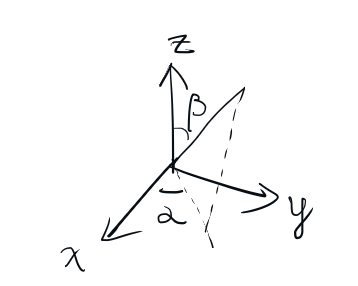
\includegraphics[width=0.4\linewidth]{pic1.png}
\end{figure}

So in this case, we have
\begin{align*}
    \ket{\vb{n}} = e^{-iS_y\gamma/\hbar}\ket{+} &=
    e^{-i\sigma_y\gamma/2} \begin{pmatrix}
        1 \\ 0
    \end{pmatrix} =
    \left(\cos(\gamma/2)-i\sigma_y\sin(\gamma/2)\right)
    \begin{pmatrix}
        1 \\ 0
    \end{pmatrix} \\
    &= \begin{pmatrix}
    \cos(\gamma/2) \\ \sin(\gamma/2)
    \end{pmatrix}
\end{align*}

The eigenstate of $S_x$ with eigenvalue $\hbar/2$ is $ \begin{pmatrix}
    1/\sqrt{2} \\ 1/\sqrt{2}
\end{pmatrix}$ (setting $\gamma=\pi/2$), so the probability getting
$\hbar/2$ when measuring $S_x$ is:
\begin{equation}
    \lvert 
    \begin{pmatrix}
        1/\sqrt{2} & 1/\sqrt{2}
    \end{pmatrix}\vdot \begin{pmatrix}
        \cos(\gamma/2) \\ \sin(\gamma/2)
    \end{pmatrix}
    \rvert^2
    = \frac{1}{2}(\cos(\gamma/2)+\sin(\gamma/2))^2
\end{equation}
Also, the dispersion is
\begin{align*}
    \braket{(S_x-\braket{S_x})^2} 
    &= \braket{S_x^2} - \braket{S_x}^2
    \\
    &=
    \begin{pmatrix}
        \cos(\gamma/2) & \sin(\gamma/2)
    \end{pmatrix}
    \vdot
    \hbar^2/4 \sigma_x^2
    \begin{pmatrix}
        \cos(\gamma/2) \\ \sin(\gamma/2)
    \end{pmatrix}
    -
    \left[
    \begin{pmatrix}
        \cos(\gamma/2) & \sin(\gamma/2)
    \end{pmatrix}
    \vdot
    \hbar/2 \sigma_x
    \begin{pmatrix}
        \cos(\gamma/2) \\ \sin(\gamma/2)
    \end{pmatrix}
    \right]^2
    \\
    &=
    \sin ^2\left(\frac{\gamma}{2}\right)+\cos
    ^2\left(\frac{\gamma}{2}\right)-4 \sin ^2\left(\frac{\gamma}{2}\right)
    \cos ^2\left(\frac{\gamma}{2}\right)
    \\
    &=
    1-\sin^2(\gamma) = \cos^2(\gamma)
\end{align*}
\end{document}
